\documentclass{beamer}

% Theme choice (you can change this to your preference)
\usetheme{Madrid}
\usecolortheme{dolphin}
\usepackage{amsmath, amssymb}
\usepackage{hyperref}
\usepackage{graphicx}
\usepackage{booktabs} % For better tables
\usepackage{caption}

% Title Page Details
\title{Code Verification via the Method of Manufactured Solutions}
\author{Marvyn Bailly}
\date{\today}

\begin{document}

% Title Slide
\begin{frame}
    \titlepage
\end{frame}

% Section: Motivation
\section{Motivation}

% Motivation Slide 1
\begin{frame}{Motivation}
    \begin{itemize}
        \item \textbf{Challenges in Numerical Simulations:}
            \begin{itemize}
                \item Numerical codes are complex, can be long, and prone to subtle bugs.
                \item Identifying these bugs can be time-consuming and difficult.
            \end{itemize}
        \item \textbf{Importance of Verification:}
            \begin{itemize}
                \item Ensuring that the numerical method accurately solves the intended mathematical model.
                \item Verification provides confidence in the simulation results.
            \end{itemize}
    \end{itemize}
\end{frame}


% Section: Code Verification
\section{Code Verification}

% Code Verification Slide 1
\begin{frame}{Code Verification}
    \begin{itemize}
        \item \textbf{Primary Goal:}
            \begin{itemize}
                \item To convincingly demonstrate that the numerical code accurately solves the PDE with the prescribed initial and boundary conditions.
            \end{itemize}

            \item \textbf{Note:}
            \begin{itemize}
                \item Code verification does not inherently debug the code.
            \end{itemize}
    \end{itemize}
\end{frame}

% Motivation Slide 2
\begin{frame}{Motivation: Verification Difficulties}
    \begin{itemize}
        \item \textbf{Difficulties:}
            \begin{itemize}
                \item Some numerical methods may exhibit obvious failures.
                \item Conversely, other methods might appear to perform well visually but still produce inaccurate results.
            \end{itemize}
    \end{itemize}
    \vspace{0.5cm}
    \begin{figure}[h]
        \centering
        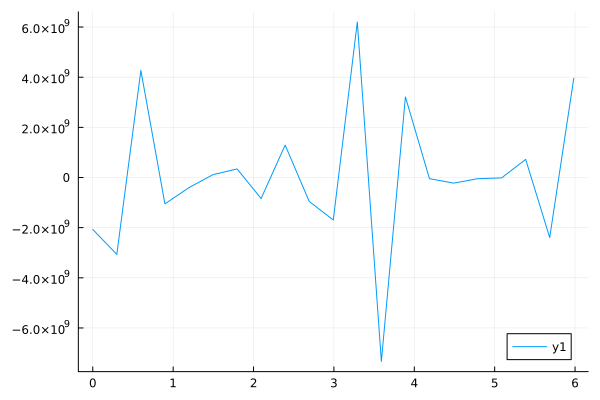
\includegraphics[width=0.45\textwidth]{images/blowup_example.png}
        \hspace{0.05\textwidth}
        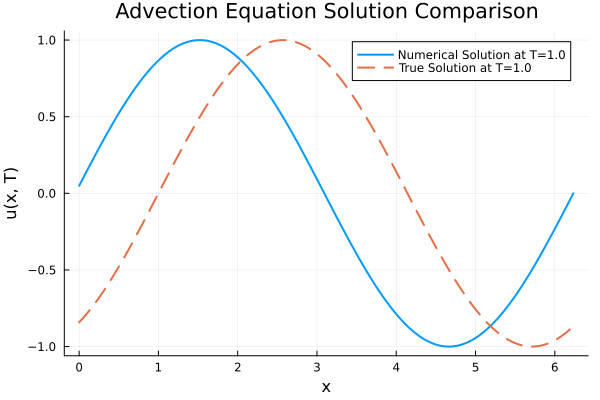
\includegraphics[width=0.45\textwidth]{images/advection_solution.png}
        \caption{Left: Method Failing (Blowing Up) \quad Right: Method Appearing Correct}
        \label{fig:motivation_graphs}
    \end{figure}
    \vspace{-0.5cm}
\end{frame}


% Code Verification Slide 2
\begin{frame}{Code Verification: Most Convincing Method}
    \begin{itemize}
        \item \textbf{Using Known True Solutions:}
            \begin{itemize}
                \item Analytical solve the PDE to find the true solution and compare against the numerical result. 
            \end{itemize}
        \item \textbf{Limitations:}
            \begin{itemize}
                \item True solutions are not always available, especially for complex or nonlinear PDEs.
            \end{itemize}

    \end{itemize}
\end{frame}

% Section: Method of Manufactured Solutions (MMS)
\section{Method of Manufactured Solutions (MMS)}

% MMS Slide 1
\subsection{Introduction to MMS}

\begin{frame}{Method of Manufactured Solutions (MMS)}
    \begin{itemize}
        \item \textbf{Concept Overview:}
            \begin{itemize}
                \item MMS is a technique for code verification when the analytical solution is not unavailable.
                \item It involves "manufacturing" a solution and modifying the original PDE to incorporate this solution.
                \item Solve the modified PDE numerically and compare the numerical solution to the manufactured solution.
            \end{itemize}
    \end{itemize}
\end{frame}

% MMS Slide 2
\begin{frame}{MMS: Theoretical Framework}
    \begin{itemize}
        \item \textbf{Original PDE:}
            \[
                \mathcal{L}(u(t,\mathbf{x})) = 0
            \]
            where $\mathcal{L}$ is a differential operator representing the PDE.
        \item \textbf{Manufactured Solution:}
            \[
                U(t,\mathbf{x})
            \]
            A user-defined solution that may not satisfy the original PDE.
        \item \textbf{Determining the Source Term:}
            \[
                \mathcal{L}(U(t,\mathbf{x})) = Q(t,\mathbf{x})
            \]
            By substituting $U(t,\mathbf{x})$ into the PDE, we derive the source term $Q(t,\mathbf{x})$.
        \item \textbf{Modified PDE:}
            \[
                \mathcal{L}(u(t,\mathbf{x})) = Q(t,\mathbf{x})
            \]
            Now, $U(t,\mathbf{x})$ is an exact solution to the modified PDE.
    \end{itemize}
\end{frame}

% Section: Example
\section{Example}

\subsection{Advection Equation Example}

\begin{frame}{Example: Advection Equation}
    \textbf{1D Advection Equation:}
    \begin{equation} \label{1}
        \mathcal{L}(u) \equiv u_t + a u_x = 0
    \end{equation}
    \begin{itemize}
        \item \textbf{Manufactured Solution:}
        \[ 
            U(t,x) = \cos(t) + \sin(x)
        \]
        \item \textbf{Source Term:}
        \[
            \mathcal{L}(U) \equiv -\sin(t) + a\cos(x) = Q(t,x)
        \]
    \end{itemize}
    \textbf{Modified Advection Equation}
        \[
            \mathcal{L}(u) = Q(t,x) \quad\text{or}\quad u_t + a u_x = -\sin(t) + a\cos(x) 
        \]
\end{frame}

% Section: Guidelines for Creating Manufactured Solution
\section{Guidelines for Creating Manufactured Solutions}

\begin{frame}{Guidelines for Creating Manufactured Solutions}
    \begin{itemize}
        \item \textbf{Generality:}
            \begin{itemize}
                \item Ensure the manufactured solution is sufficiently general to exercise all terms in the governing PDE.
                \item E.g., Equation \ref{1} requires a solution with $x$ and $t$ dependence.
            \end{itemize}
        \item \textbf{Non-Triviality:}
        \begin{itemize}
            \item The solution should involve non-trivial derivatives to ensure all terms in the PDE are active.
            \item E.g., Linear solutions will not suffice for verifying 2nd-order PDEs.
        \end{itemize}
        \item \textbf{Compliance with PDE Assumptions:}
            \begin{itemize}
                \item The solution must adhere to the inherent assumptions of the PDE.
                \item E.g., if the PDE is defined for positive times, the solution should be valid for $t > 0$.
            \end{itemize}
        \item \textbf{Physical Realism:}
            \begin{itemize}
                \item The manufactured solution does not need to be physically realistic.
            \end{itemize}
    \end{itemize}
\end{frame}

% Section: Initial and Boundary Conditions
\section{Initial and Boundary Conditions}

\begin{frame}{Initial and Boundary Conditions}
    \begin{itemize}
        \item \textbf{Initial Conditions:}
            \begin{itemize}
                \item The manufactured solution does not need to satisfy the original initial condition for the PDE.
            \end{itemize}
        \item \textbf{Boundary Conditions:}
            \begin{itemize}
                \item The boundary conditions can be challenging.
                \item Design different manufactured solutions to test different types of boundary conditions.
            \end{itemize}
        \item \textbf{Current Implementation}
            \begin{itemize}
                \item Requires initial condition for manufactured solution to match original initial condition. 
                \item Requires boundary conditions to be periodic.  
            \end{itemize}
    \end{itemize}
\end{frame}

\begin{frame}{Example: Advection Equation}
    \textbf{Initial Condition}
    \[
        u(0,x) = f(x) = \sin(x)
    \]
    \begin{itemize}
        \item \textbf{Manufactured Solution:}
        \[ 
            \tilde{U}(t,x) = \cos(t) + \sin(x)
        \]
        but
        \[ 
            \tilde{U}(0,x) = 1 + \sin(x) \neq f(x)
        \]
        so take
        \[ 
            U(t,x) = - 1 + \cos(t) + \sin(x)
        \]
    \end{itemize}
\end{frame}

% MMS Slide 3
\subsection{Applying MMS}

\begin{frame}{Applying MMS for Code Verification}
    \begin{itemize}
        \item \textbf{Verification Process:}
            \begin{itemize}
                \item Set up the modified PDE for numerical solving.
                \item Run the numerical solver to obtain the numerical solution $v(t,\mathbf{x})$.
                \item Compare $v(t,\mathbf{x})$ with the manufactured solution $U(t,\mathbf{x})$.
            \end{itemize}
        \item \textbf{Order of Accuracy:}
            \begin{itemize}
                \item Evaluate whether the numerical method achieves the expected order of accuracy when refining the mesh.
                \item Consistency in the order of accuracy between the original and modified PDEs confirms the correctness of the numerical implementation.
            \end{itemize}
    \end{itemize}
\end{frame}

% Section: Understanding Accuracy
\section{Understanding Accuracy}

\begin{frame}{Reminder: What is Accuracy?}
    \textbf{Accuracy in Numerical Methods:}
    \begin{itemize}
        \item Accuracy measures how closely the numerical solution approximates the exact solution.
        \item For a method with order of accuracy \( p \), the global error \( E \) typically scales with the grid spacing \( h \) as:
        \[
            E \propto h^p
        \]
        \item \textbf{Higher Order = Greater Accuracy:} As \( p \) increases, the numerical solution converges to the exact solution more quickly as the grid is refined.
        \item \textbf{Practical Meaning:} For example, a second-order method (with \( p = 2 \)) will reduce its error by roughly a factor of \( 4 \) when the grid spacing \( h \) is halved.
    \end{itemize}
\end{frame}

% Section: Approximating Accuracy
\section{Approximating Accuracy}

\begin{frame}{Approximating Accuracy}
    \begin{itemize}
        \item \textbf{Procedure:}
            \begin{enumerate}
                \item Conduct simulations using two different grid resolutions: $h$ and $h/r$, where $r$ is the refinement ratio.
                \item Compute the global errors $E_1$ and $E_2$ corresponding to each grid size respectively.
                \item For a $p$th-order method, we expect
                \[
                    E_1 \approx C_1 h^p \text{ and } E_2 \approx C_2 \left(\frac{h}{r}\right)^p
                \]
                \item Calculate the observed order of accuracy $p$
                    \[
                        p \approx \frac{\log{\left(\frac{E_1}{E_2}\right)}}{\log{r}}
                    \]
                \end{enumerate}
            \item Note: This is a rough approximation. 
    \end{itemize}
\end{frame}


% Section: Implementation
\section{Implementation}

\subsection{Pseudocode}

\begin{frame}{Implementation}
    \textbf{Handling the Source Term:}
    \begin{itemize}
        \item The source term \( Q(x,t) \) can become quite complex depending on the PDE and manufactured solution.
        \item To simplify this process:
        \begin{itemize}
            \item Solve for \( Q(x,t) \) symbolically.
            \item Convert symbolic \( Q(x,t) \) into a forcing term for numerical solver.
        \end{itemize}
    \end{itemize}
    \textbf{Language Choice:}
    \begin{itemize}
        \item This approach requires a language capable of both symbolic manipulation, code generation and code execution.
    \end{itemize}
\end{frame}

\begin{frame}{Forcing Terms Can Get Complex}
    \textbf{Example of a Complex Forcing Term:}
    \begin{figure}[h]
        \centering
        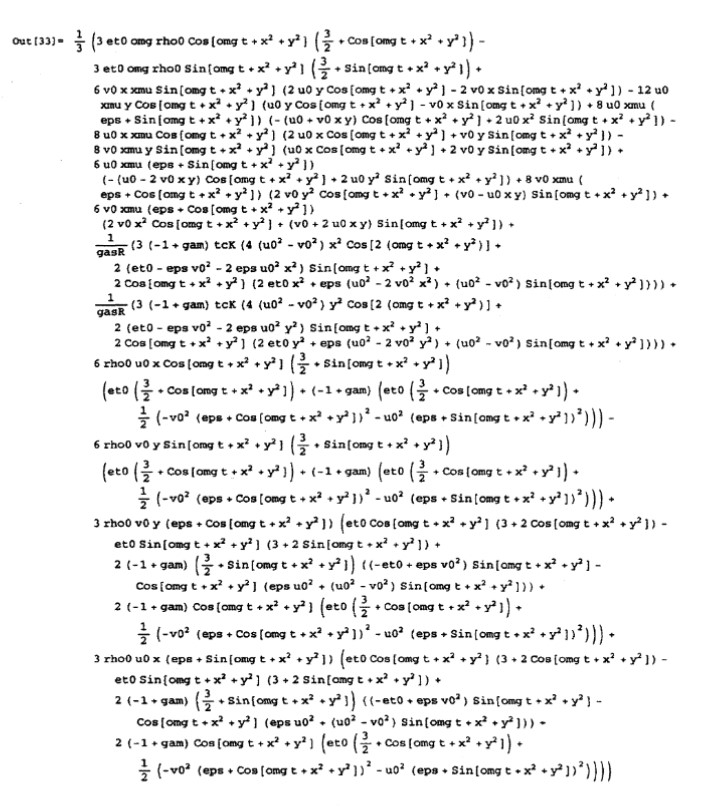
\includegraphics[width=0.50\textwidth]{images/ew.png}
        \caption{Source term for 2-D laminar compressible Navier-Stokes equations}
    \end{figure}
    \vspace{0.5cm}
\end{frame}

\begin{frame}{Python vs Julia}
    \begin{itemize}
        \item \textbf{Symbolic Computation:} 
            \begin{itemize}
                \item Both Python and Julia offer symbolic computation capabilities through their respective libraries, SymPy and Symbolics.jl.
                \item Symbolics.jl can export expressions as optimized C++.
            \end{itemize}

        \item \textbf{Pros of Julia:} 
            \begin{itemize}
                \item Julia compiles code using Just-in-Time compilation, allowing it to achieve speeds comparable to languages like C.
                \item Julia is designed with numerical and scientific computing in mind.
                \item Julia offers built-in support for parallel and distributed computing.
            \end{itemize}

        \item \textbf{Cons of Julia:} 
            \begin{itemize}
                \item Julia's library ecosystem is limited compared to Python's. 
                \item Julia's community and available resources are smaller compared to Python
            \end{itemize}
    \end{itemize}
\end{frame}

\begin{frame}{Implementation: Pseudocode}
    \textbf{Procedure:}
    \begin{enumerate}
        \item User specifies the PDE and a manufactured solution \( U(x,t) \) in Julia.
        \item User specifies where to place forcing term using comments
        \item Symbolically solves for the source term \( Q(x,t) = \mathcal{L}(U(x,t)) \)
        \item \( Q(x,t) \) is written to the numerical solver as a forcing term
        \item Run the numerical solver for two different mesh sizes
        \item Approximate order of accuracy
    \end{enumerate}
    \vspace{0.5cm}
    \begin{itemize}
        \item \textit{Let's see it in action!}
    \end{itemize}
\end{frame}


% Section: Code and Simple Example
\section{Code and Simple Example}

\begin{frame}{Code and Simple Example}
    \textbf{Numerical Test Setup:}
    \begin{itemize}
        \item \textbf{Equation:} 1D advection equation $\mathcal{L}(u) \equiv u_t + 4 u_x = 0$
        \item \textbf{Initial Condition:} $u(x,0) = \sin(x)$.
        \item \textbf{Boundary Conditions:} $2\pi$-periodic.
        \item \textbf{Manufactured Solution:} $U(x,t) = e^{xt}cos(t)sin(x)$
        \item \textbf{Numerical Method:} Lax-Wendroff scheme (second order) 
    \end{itemize}
\end{frame}

% Slide 2: Diffusion Equation with Manufactured Solution
\begin{frame}{Oceananigans Example}
    \textbf{PDE: Diffusion Equation}
    \begin{equation*}
        \frac{\partial u}{\partial t} = \kappa \frac{\partial^2 u}{\partial x^2} + f(x, t),
    \end{equation*}
    subject to
    \begin{equation*}
        u(x,0) = e^{\frac{-x^2}{2w^2}}
    \end{equation*}
    where:
    \begin{itemize}
        \item \( u(x, t) \): Scalar field (temperature).
        \item \( \kappa \): Diffusion coefficient.
        \item \( w \): Width of Guassian.
        \item \( f(x, t) \): Forcing term derived from the manufactured solution.
    \end{itemize}
\end{frame}


% Section: Future Plans
\section{Future Plans}

\begin{frame}{Future Plans}
    \begin{itemize}
        \item \textbf{Expand Boundary Condition Types:}
            \begin{itemize}
                \item Incorporate various boundary conditions such as Dirichlet and Neumann to test the robustness of numerical methods.
            \end{itemize}
        \item \textbf{Enhance Code Verification:}
        \begin{itemize}
            \item Implement verification between Julia and C++ code.
        \end{itemize}
        \item \textbf{Increase PDE Complexity:}
            \begin{itemize}
                \item Apply MMS to more complex PDEs, aiming to verify the implementation of Navier-Stokes equations!
            \end{itemize}
        \item \textbf{Generalize Manufactured Solutions:}
            \begin{itemize}
                \item Allow users to define manufactured solutions on diverse subsets of 2-D and 3-D space.
            \end{itemize}
        \item \textbf{Make a Library:}
        \begin{itemize}
            \item Create a MMS library for users to download for general verification.
        \end{itemize}
    \end{itemize}
\end{frame}



% Section: References
\section{References}

\begin{frame}[allowframebreaks]{References}
    \bibliographystyle{apalike}
    \begin{thebibliography}{10}
        \beamertemplatearticlebibitems
        \bibitem{Roache2002CodeVB}
        P.~J. Roache.
        \newblock {Code Verification by the Method of Manufactured Solutions}.
        \newblock {\em Journal of Fluids Engineering - Transactions of the ASME}, 124:4--10, 2002.
        \newblock Available: \url{https://api.semanticscholar.org/CorpusID:121230632}
        
        \beamertemplatearticlebibitems
        \bibitem{Symbolics.jl}
        Symbolics.jl Documentation.
        \newblock \url{https://symbolics.juliasymbolics.org/}


    \end{thebibliography}
\end{frame}




\end{document}
